\documentclass[a4paper]{article}

\usepackage{lmodern}

%% Language and font encodings
\usepackage[french]{babel}
\usepackage[utf8x]{inputenc}
\usepackage[T1]{fontenc}

%% Sets page size and margins
\usepackage[a4paper,top=3cm,bottom=3cm,left=2cm,right=2cm,marginparwidth=2cm]{geometry}
%% Useful packages
\usepackage{amsmath}
\usepackage{graphicx}
\usepackage[colorinlistoftodos]{todonotes}
\usepackage[colorlinks=true, allcolors=black]{hyperref}
\usepackage{fourier-orns}
\usepackage{titlesec}
\usepackage{fancyhdr}
\usepackage{fancyvrb}
%\renewcommand{\thefootnote}{\*}
\pagestyle{fancy} 
\setcounter{tocdepth}{5}



%% Tikz stuff
\usepackage{tikz}
\usetikzlibrary{calc, arrows}
\tikzstyle{incolore} = [rectangle, rounded corners, draw=black, minimum height=1cm, minimum width=3cm, text width=3cm, text centered]
\usepackage{float}


\usepackage{libertine}
\newcommand{\hsp}{\hspace{20pt}}
\newcommand{\HRule}{\rule{\linewidth}{0.5mm}}





\renewcommand{\headrulewidth}{1pt}
\fancyhead[C]{} 
\fancyhead[L]{}
\fancyhead[R]{\footnotesize{\leftmark}}

\renewcommand{\footrulewidth}{1pt}
\fancyfoot[C]{} 
\fancyhead[L]{}
\fancyfoot[R]{\thepage}

\definecolor{Zgris}{rgb}{0.87,0.85,0.85}

\usepackage{eso-pic,graphicx}
\usepackage{xcolor}
\newcommand{\bgimg}[1]{
\AddToShipoutPicture
   {
      \put(\LenToUnit{0 cm},\LenToUnit{0 cm})
      {
            \includegraphics[width=\paperwidth,height=\paperheight]{#1} 
      }
   }
}


\begin{document}


%%\bgimg{Image_15.jpg}





  \begin{titlepage}
    \begin{sffamily}
    \begin{center}
      \textnormal{}\\[6.5cm]
      % Upper part of the page. The '~' is needed because \\
      % only works if a paragraph has started.
      % Title
      \HRule \\[0.4cm]
      { \Huge \bfseries Synthèse\\ Architecture des ordinateurs Q2\\ [0.4cm] }
      \HRule \\[3cm]
      \Large
      Premier Bloc\\
      Sécurité des systèmes\\
      Année académique 2019-2020\\[0.2cm]
      \emph{Rédigé par Sénéchal Julien}
      \vfill
      % Bottom of the page
      {\large 28 Mai 2020}
    \end{center}
    \end{sffamily}
  \end{titlepage}

  \section{La virtualisation}
    \subsection{Avantages}

      \begin{itemize}
      \item Meilleure utilisation du CPU
      \item Economie en surface et en électricitée
      \item Load Balancing (changer la charge d'un serveur si celui-ci est trop surchargé)
      \item Tolérance aux pannes
      \item Isolation
      \item Peut servir a déboguer des programmes (ne pas planter l'OS principal)
      \item Développement logiciel
      \item Compatibilitée avec un ancien systèmes
      \item Virtualisation hétérogène
      \item Affectation des ressources a chaud
      \end{itemize}

    \subsection{Contraintes}

      \begin{itemize}
        \item Pas de self-service (Gestion par Admin)
        \item Surchage du travail du CPU
          \begin{itemize}
            \item Solution: containers 
          \end{itemize}
      \end{itemize}
    
    \subsection{Methode de virtualisation}

      \begin{itemize}
        \item Hyperviseur (Hyperviseur de Type I)
        \begin{itemize}
          \item Intermédiaire direct entre le matériel et les OS Virtualisés
          \item Tourne en espace kernel (rôle de l'OS)
        \end{itemize}

        \item Modèle hôte invité (Hyperviseur de Type II)
        \begin{itemize}
          \item VMM (Manager de machine virtuelle) exécuté en espace utilisateur (application) $\Rightarrow$ VM dans l'espace utilisateur.
          \\Résultat :
          + lent et + facile a mettre en place
        \end{itemize}
        \item Dans les 2 cas, le VMM doit donner l'illusion a l'OS invité qu'il a l'accès aux ressources de matériel
      \end{itemize}

    \subsection{Technologies de virtualisation}

      \begin{itemize}
        \item Matériel
        \begin{itemize}
          \item Le matériel fournit un support permettant de faciliter la consctruction d'un VMM et de pouvoir isoler les OS invités.\\
          Exemple :
        \begin{itemize}
          \item Pour processeur AMD : AMD-V
          \item Pour un processeur Intel : VT-x
          \item Etc...
        \end{itemize}
        \end{itemize}
        \item Logiciel
        \begin{itemize}
          \item Full virtualisation : Création de faux matériel par l'hyperviseur, auxquels l'OS invité a accès. 
          (L'OS invité doit être de la même architecture que le processeur physique : x86, x64, etc...)
          \item Emulation : Création d'un environnement virtuel complet (même le CPU avec une architecture différente) $\rightarrow$ Basses performance
          \item Paravirtualisation : L'OS invité sait qu'il est dans une machine virtuelle (peut communiquer directement avec l'hyperviseur)
          \item Virtualisation assistée par le matériel (HVM) : 
          \begin{itemize}
            \item Ajout d’extension de virtualisation au processeur
            \item Plus d'emulation de mémoire
            \item Gestion de leur propre interruptions/contexte par les VM elles-mêmes
            \item Accès direct au processeur
          \end{itemize}
          \item Isolation : Spécificitée UNIX ! Permet d'isoler une application du reste du monde.
          \item Container :
          \begin{itemize}
            \item Pas d'emulation matériel
            \item Un répertoire = un OS
            \item Pas de noyau
            \item Exemple : Dockers
          \end{itemize}
        \end{itemize}

      \end{itemize}

      \begin{figure}[H]
        \centering
        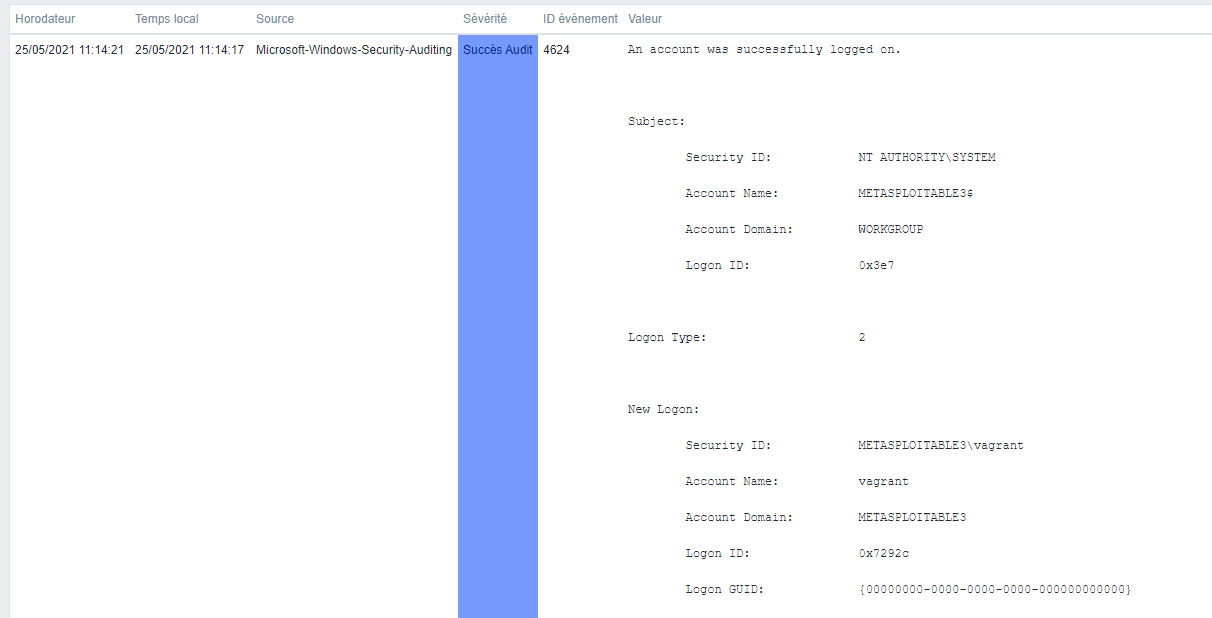
\includegraphics[width = 0.5\textwidth]{images/1.PNG}
        \caption{Résumé des différents types de virtualisation}
      \end{figure}

    \subsection{Privilèges d'accès}
    
    \begin{itemize}
      \item L'OS hôte accède directement au matériel
      \item Niveau de privilège :
      \begin{itemize}
        \item Mécanisme interne au CPU qui empêche une application d'usurper d'identitée d'un OS hôte
        \item \emph{Rings Levels}
        \begin{itemize}
          \item Exemple : 0 = le plus privilégié = OS hôte
          \item Le nombre de niveau dépends de l'architecture du CPU
          \item \emph{Ring 3} - User level : Le code est exécuté directement par le CPU mais il ne peut pas accéder directement a la mémoire ou au matériel
          \item \emph{Ring 0} - Kernel Level : Accès complet
          \item L'OS invité ne vera jamais qu'il n'est pas en \emph{Ring 0}. Pour cela, lorsqu'un programme veut exécuter une instruction pour laquelle il n'a pas de privilège
          suffisant, une exception va être créé (\emph{trap}), et l'hyperviseur qui écoute chaque \emph{trap} des machines va intercepter les exceptions et reprendre la main 
          en émulant le comportement attendu par la machine invitée.
          \item Shadow Structure : mécanisme pour cacher et gérer l'accès aux informations privilégié (copie privée propre a la VM)
        \end{itemize}
        
      \end{itemize}
    \end{itemize}
    
    \subsection{Virtualisation de la mémoire}

    \begin{itemize}
      \item VMM
      \begin{itemize}
        \item Partage mémoire physique
        \item Allocation dynamique
      \end{itemize}
      \item Présentation de la mémoire a un OS :
      \begin{itemize}
        \item La VM voit un espace mémoire non réel
        \item Gestion d'une table de correspondance sur la RAM entre les pages\footnote{\emph{Voir "la pagination" en cours de Système d'exploitation}} mémoire de la machine virtuelle
        et les pages physique des ressources matériel. 
      \end{itemize}
      \item Virtualisation de la MMU (Memory Management Unit)
      \begin{itemize}
        \item Shadow page table
        \begin{itemize}
          \item 2 associations dans cette table : LA VM $\rightarrow$ PA VM (créé par l'OS invité) \& PA VM $\rightarrow$ Adresse machine - MA (créé par le VMM)
          \item Une seule table d'association entre la mémoire virtuelle et la MMU de la machine ce qui est presque aussi rapide qu'en natif.
        \end{itemize}
        \item Hardware
        \begin{itemize}
          \item Extensions x86 pour la virutalisation
          \item Gain de performance : Pas de perte ou perte légère ($\pm$ 40\%)
        \end{itemize}
      \end{itemize}
    \end{itemize}

    \subsection{Cloud}
    \begin{itemize}
      \item SAAS
      \begin{itemize}
        \item Software as a service
        \item Ex: Google Doc, etc...
      \end{itemize}
      \item PAAS 
      \begin{itemize}
        \item Platform as a service
        \item Hebergement application
        \item Ex: Google Engine, Azure, etc...
      \end{itemize}
      \item IAAS 
      \begin{itemize}
        \item Infrastructure as a service
        \item Ex: OpenStack, etc...
      \end{itemize}
      \item Publique
      \begin{itemize}
        \item Via a fournisseur Cloud
        \item Ex : Amazon, RackSpace, etc...
      \end{itemize}
      \item Privé
      \begin{itemize}
        \item Cloud interne
      \end{itemize}
      \item Hybride \emph{(Mix de Privé et Publique)}
    \end{itemize}

    \subsection{Container}

    \begin{itemize}
      \item Un container $\Rightarrow$ Un OS
      \item Virtualisation au niveau de l'OS :\\ Plusieurs instances du même OS qui tournent avec le même Kernel
      \item Chaque container contient tout ce dont il a besoin
      \item Espace fournit par l'OS hôte
      \item L'OS hôte isole bien chaque container et alloue la RAM/CPU nécessaire
      \item \textbf{Avantages :}
      \begin{itemize}
        \item Facilité de déployer plusieurs instances d'une même application
        \item Isolation
        \item Performance propotionnelle a une VM
      \end{itemize}
      \item \textbf{Inconvénients :}
      \begin{itemize}
        \item Dépends de l'os
        \item Isolation moins importante qu'avec une VM
      \end{itemize}
    \end{itemize}
















  \newpage
  \section{Les ordinateurs superscalaires}
    Ordinateurs superscalaires $\Rightarrow$ Ordinateurs utilisant une puce avec plusieurs \emph{ALU} travaillant en parrallèle.\\
    \textbf{Rappel :} L'alu est l'"Arithmetic logic unit". Cette unitée gère les calculs des instructions.

    \subsection{AR2}
    \begin{itemize}
      \item 2 \emph{ALU}
      \item Execution de 2 instructions \emph{arithmétique} en parrallèle
      \item Même registre pour les 2 \emph{ALU}
    \end{itemize}
    \begin{figure}[H]
      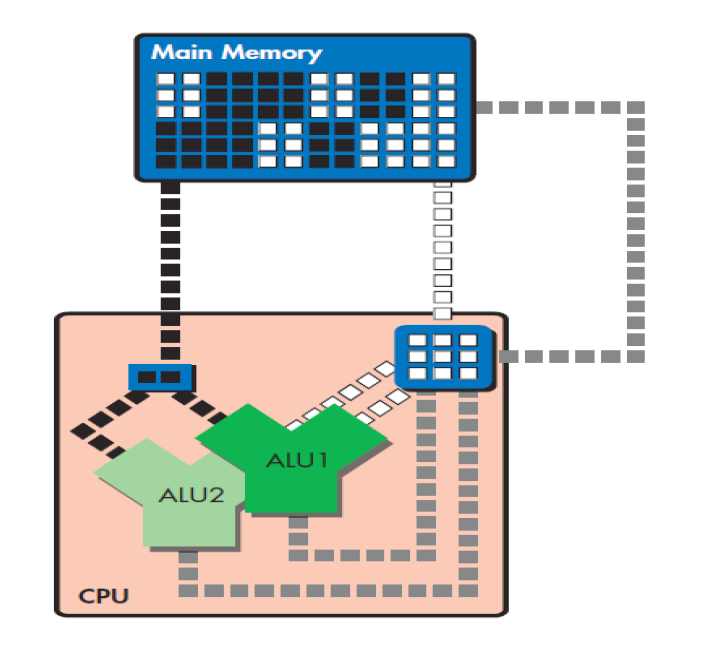
\includegraphics[width = 0.5 \textwidth]{images/2.PNG}
      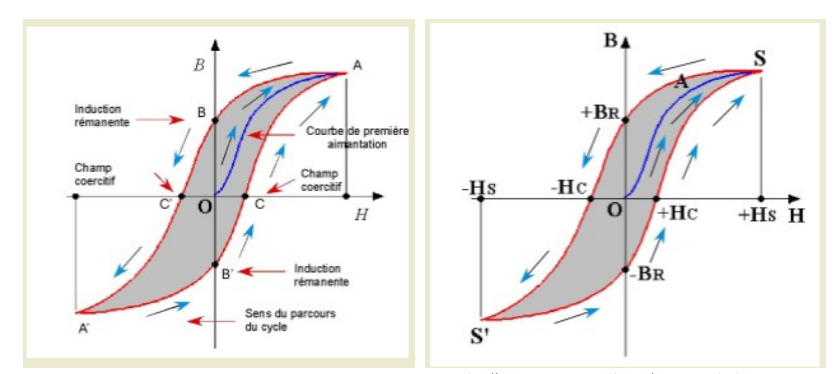
\includegraphics[width = 0.5 \textwidth]{images/3.PNG}
      \caption{Représentation AR2}
    \end{figure}

    \subsubsection{Decode/Dispatch}
    Un nouveau circuit vient de s'ajouter a ce que l'on connaissait déjà (voir \figurename{2}).\\
    Rôle :
    \begin{itemize}
      \item Déterminer si 2 instructions peuvent être réalisés simultanément
      \item Si oui, l'unitée de dispatch va répartir les 2 instructions sur les 2 ALU
      \item Si non, l’unité de dispatch les envoie dans l’ordre du programme vers le premier ALU
    \end{itemize}

    \subsubsection{Programming Model}
    \begin{itemize}
      \item Pas de changements
      \item Illusion d'une execution séquentielle pour le bien du programmeur.
    \end{itemize}

    \subsubsection{Cycle d'exécution}
    \begin{itemize}
      \item Capacité de \emph{FETCH} 2 fois simultanément
      \item Capacité de \emph{Decode/Dispatch} 2 instructions simultanément
    \end{itemize}
    \begin{figure}[H]
      \centering
      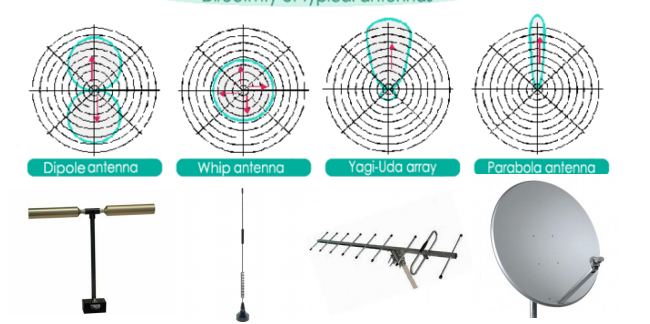
\includegraphics[width = 0.4 \textwidth]{images/4.PNG}
      \caption{Représentation du cycle de l'AR2}
    \end{figure}

    \subsection{Architecture superscalaire}
    \begin{itemize}
      \item Permet de dépasser le seuil d'une instruction par pulsation d'horloge fixée par un pipeline simple. C'est le cas du AR2 que l'on vient de traiter.
      \item + un CPU disposera d'ALU, + $\frac{instructions\ terminees}{pulsation\ d'horloge}$
    \end{itemize}

    \subsubsection{Différentes opérations arithmétique et logique}
    \begin{itemize}
      \item Opérations arithmétique : $+$, $-$, $\div$, $\times$
      \item Opérations logiques : AND, OR, NOT, XOR, shits, rotation de bits
      \item Opérations Scalaires et Vectorielles
    \end{itemize}
    Tout cela pour en venir au fait qu'on pourrait répartir spécifiquement les tâches !!!

    \subsubsection{Processeur Intel Pentium}
    Répartition des tâches de l'ALU :
    \begin{itemize}
      \item IU : Unité d'execution des entiers (Interger execution unit)
      \item FPU : Unité d'execution des virgules flottantes (Floating-point unit)
      \item LSU : Unité responsable des \emph{laod},\emph{store} et du calcul des adresses (Load-Store unit)
      \item BEU : Unité responsable sauts conditionnels et non conditionnels (Branch Execution Unit)
    \end{itemize}
    Jusqu'ici les ALU étaient une unité concrète, dorénavant, l'ALU sera un terme générique de l'ensemble des unités d’exécution faisant des opérations arithmétiques ou logiques.

    \begin{figure}[H]
      \centering
      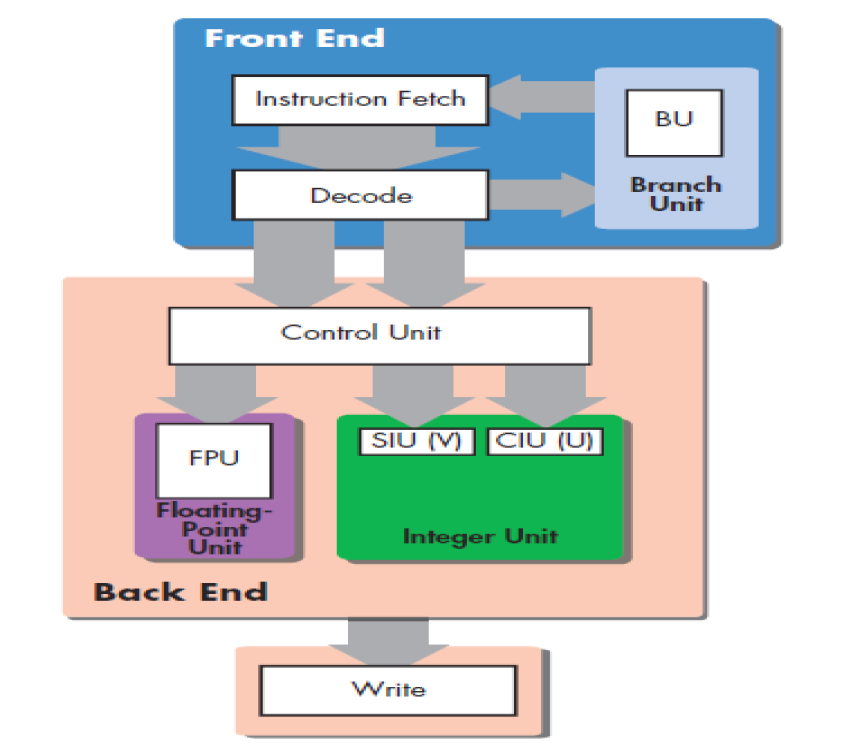
\includegraphics[width = 0.4 \textwidth]{images/5.PNG}
      \caption{Représentation de L'Intel Pentium}
    \end{figure}

    \subsubsection{Problèmes de l'architecture superscalaire}
    \begin{itemize}
      \item Certaines conditions peuvent empêcher la mise en parrallèle de plusieurs instructions arithmétiques
      \item Possibilitée de création de \emph{"bulles"} (comme vu au Q1)
      \item Exemple : 
      \begin{itemize}
        \item 1ère instruction : \emph{add A,B,C}
        \item 2ème instruction : \emph{add C,D,D}
        \item \textbf{Impossible de les réaliser simultanément}
        \item Conséquence en superscalaire : L'ALU éxecutant la 2ème instruction devra attendre que l'ALU executant la 1ère instruction finisse.
        \item Conséquence en pipeline : La 2ème instruction \emph{add} devra attendre attendre que la 1ère passe son étape \emph{write} avant de pouvoir faire son \emph{execute}
      \end{itemize}
      \item Solution :
      \begin{itemize}
        \item L'unité de Dispatch doit remarquer si 2 instructions ne peuvent pas être exécuté en même temps
        \item Une technique appellé le \emph{forwarding} consiste a prendre le résultat de la 1ère instruction a la sortie de l'ALU et de le renvoyer directement dans le 2ème ALU.
        On évite ainsi l'étape du \emph{Write}. Pour éviter les conflits, une technique est de réattribuer les registres sur des registres physiques comme on peut voir sur la \figurename{5}
      \end{itemize}

      \begin{figure}[H]
        \centering
        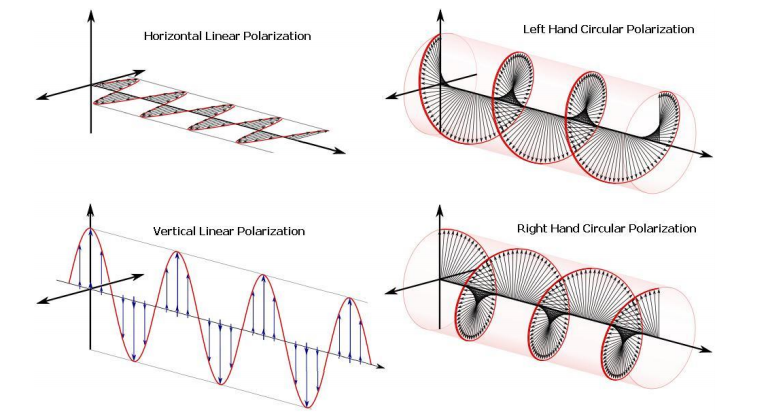
\includegraphics[width = 0.5 \textwidth]{images/6.PNG}
        \caption{Réattribution des registres}
      \end{figure}

      Exemple concret de son utilisation :
      \begin{itemize}
        \item 1ère instruction : \emph{add A,B,C}
        \item 2ème instruction : \emph{add D,B,A}
        \item Pas de dépendances dans ces 2 instructions et donc les 2 instructions peuvent s'exécuter simultanément.
        \item Problème sans réattribution des registres : \\La 2ème instruction réécrit sur le registre A qui lui est utilisé dans le calcul de la 1ère instruction.
        \item Avec réattribution des registres : \\ Pas de soucis, la 2ème instruction fait son calcul, mets le résultat dans son registre personnel temporaire. 
        Pareil pour la 1ère instruction. Et c'est seulement quand les 2 ont fini leur exécution que la valeur est écrite dans les registres du programming model.
      \end{itemize}
      
    \end{itemize}

    \subsubsection{Problèmes liés a la structure du CPU}
    \begin{itemize}
      \item Il est nécessaire de faire des modifications pour que les 2 ALU puissent accéder simultanément au registre
      \item Solution :
      \begin{itemize}
        \item Regrouper tous les registres en une unité spéciale $\rightarrow$ le fichier de registre. Il est accèssible par un bus de données et par 2 ports (Input/Output) 
        \item Chaque ALU est connecté à cette unité à l'aide de 2 ports de lecture permettant la lecture simple de 2 registres simultanément et d'un port d'écriture.
      \end{itemize}
    \end{itemize}

    \subsubsection{Problèmes liés aux instructions de saut}
    Avant, il fallait attendre pendant que l'instruction de saut était évaluée et donc ne pas continuer le pipeline... Ce qui créait des bulles

    Maintenant, la solution est une technique appelé la \emph{prédiction de branchement} qui contourne ce bloquage. 
    Une fois que l'adresse de la prochaine instruction connue, l'attente du chargement de la prochaine instruction peut prendre du temps ! 
    A nouveau une technique appelé \emph{instruction caching} permet de réduire ce temps d'attente.










  \section{RISC-CISC}
  Pour des raisons évidentes, il fallu passer d'un mode où chaque programme était intimement lié au hardware a un mode d'utilisation où l'ISA (Instruction Set Architecture) joue le
  rôle d'intermédiaire entre le Hardware et le Software.

  \begin{figure}[H]
    \centering
    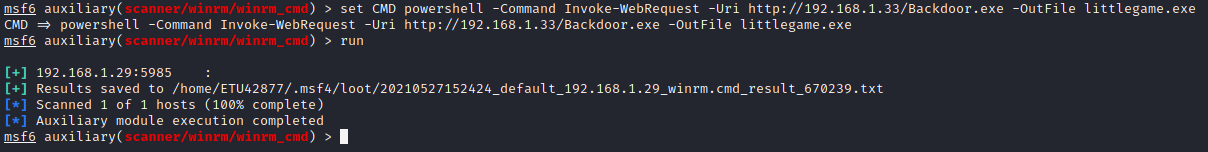
\includegraphics[width = 0.3 \textwidth]{images/7.PNG}
    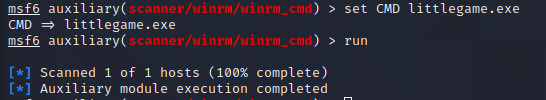
\includegraphics[width = 0.4 \textwidth]{images/8.PNG}
    \caption{Création de l'ISA}
  \end{figure}

  On a alors mis en place le \emph{microcode engine} pour assurer cette abstraction. Il s'agissait de une mémoire ROM stockant des microcodes programs et une unité d’exécution 
  qui exécute ces programmes.\\[0.2cm]
  Fonctionnement :
  \begin{itemize}
    \item L'unité microcode lit l'instruction a exécuter
    \item Elle trouve alors le code dans la mémoire ROM qui correspond a cette instruction
    \item L'exécution de cette instruction produit une séquence d'instruction dans la "langue" du processeur
  \end{itemize}
  Ce mode de fonctionnement s'appelle l'\emph{emulation} !

  Grâce a cela, a l'appartition d'une nouvelle génération de processeur, les fabricants n'avaient qu'a réécrire un microcode pour que l'ISA de l'utilisateur ne change pas.

  Au fil du temps, de plus en plus d'instruction on été ajoutée, mais toutes n'étaient pas utilisées et plus d'instriction 
  signifiait plus de ROM pour le microcode et des CPU plus volumineux et plus energivore.

  \subsection{RISC}
    On se débarrasse de tout ce qui est superflu :
    \begin{itemize}
      \item diminuer le nombre d'instruction
      \item diminuer la complexité des instructions
    \end{itemize}
    But :
    \begin{itemize}
      \item ISA plus léger
      \item Plus rapide
      \item Plus facile a implémenter dans le hardware (sans microcode engine)
    \end{itemize}

    L'énorme avantage de l'ISA n'as pas été oublié pour autant :
    \begin{itemize}
      \item Pour pouvoir se libérer su microcode engine, les machines RISC ont pu
      s’appuyer sur les progrès des compilateurs des
      langages de haut niveau. Migration du hardware vers le software
    \end{itemize}

  \subsection{CISC}
  CISC est un terme créé à postériori pour distinguer les anciennes méthodes des « nouvelles » pensées RISC.
















  \section{Pentium}
    \subsection{Mémoire cache}
    Un transfert de données entre la mémoire centrale (RAM) et les registres se fait sur une quantité énorme de cycle horloge $\Rightarrow$ apparition de la mémoire cache.
    \begin{itemize}
      \item Petite quantité de mémoire entre les registres et la mémoire centrale (RAM)
      \item Rapide
      \item Coûteuse
    \end{itemize}
    \begin{figure}[H]
      \centering
      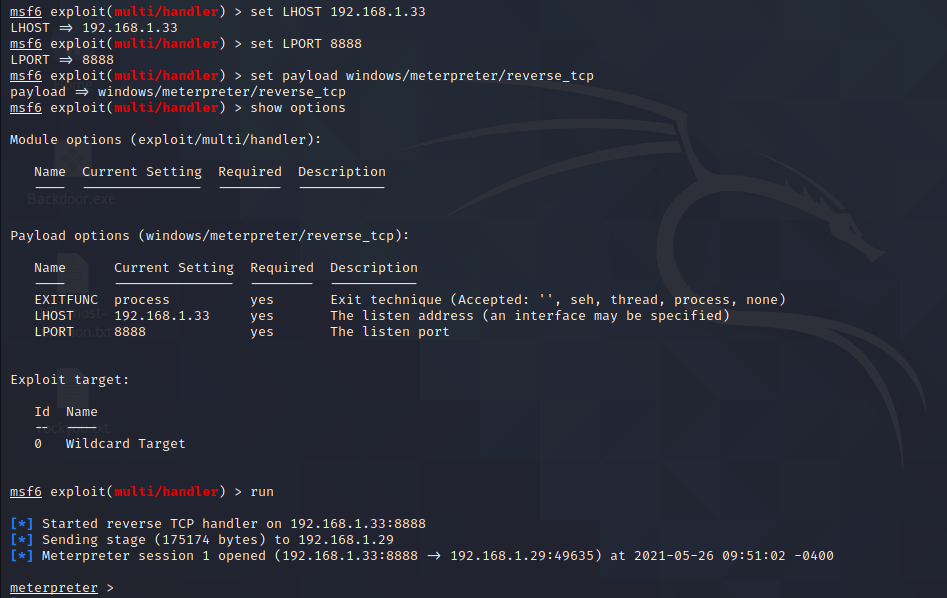
\includegraphics[width = 0.5 \textwidth]{images/9.PNG}
      \caption{Hiérarchie de la mémoire}
    \end{figure}
    
    \begin{itemize}
      \item Contient des portions de code et de données fréquemment utilisées
      \item Proche du processeur
      \item Il peut exister plusieurs niveaux de cache mémoire :
      \begin{itemize}
        \item Cache L1 : La plus petite, la plus chère, la plus proche du processeur
        \item Cache L2 : Fréquemment utilisé, entre la L1 et la mémoire centrale
        \item Cache L3 : Placé entre la L2 et la mémoire centrale. Moins fréquent
      \end{itemize}
      \item Quand le processeur a besoin de données (ou de code), il vérifie le cache L1 et si ça réussit, il place les données dans le \emph{fetch}. 
      Si ça échoue, il va vérifier dans le cache L2, copier ce dont il a besoin en cache L1 puis être transmis au Fetch, pareil pour le cache L3 en passant par L2, puis L1, etc...
      Si le contenu désiré ne se trouve dans aucun cache, le processeur va le chercher dans la mémoire centrale et le place dans les cache.
    \end{itemize}
    Organisation du cache L1 :
    \begin{itemize}
      \item 2 parties stockées séparément :
      \begin{itemize}
        \item 50\% instruction cache (codes)
        \item 50\% data cache (données)
      \end{itemize}
      \item Plus performant
    \end{itemize}
    Situation :
    \begin{itemize}
      \item Avant : sur le bus de mémoire reliant le processeur a la mémoire centrale
      \item Maintenant : les caches L1 et L2 font partie du CPU lui-même
    \end{itemize}
    
    \subsection{Pipeline du Pentium}
    Toutes les étapes des pipelines sont toujours les mêmes, sauf pour l'étape \emph{execute} qui est spécifique selon l'instruction.
    \begin{figure}[H]
      \centering
      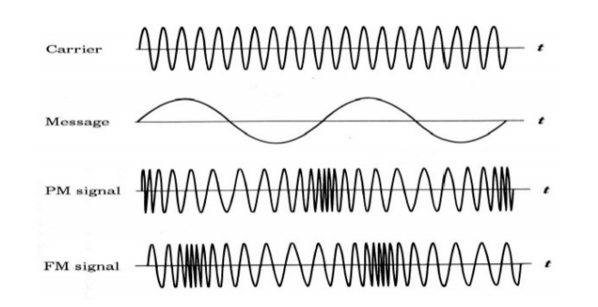
\includegraphics[width = 0.3 \textwidth]{images/10.PNG}
      \caption{Pipeline du Pentium}
    \end{figure}

    Comme la taille des instructions x86 étaient variables, nécessité de les charger dans un tampon où leurs limites sont détectées.

    \emph{Decode} est découpé en 2 parties :
    \begin{itemize}
      \item Decode-1 : Conversion de l'instruction en "language" du Pentium et détermination de si il s'agit d'une instruction de "branchement" (jump)
      \item Decode-2 : Comme l'ISA x86 permet des modes d'adressages multiples, besoin de plus de calcul d'adressage et c'est là qu'il les fait, et il décode aussi 
      les instructions plus longues grâce a une microprogrammation ROM.
    \end{itemize}

    \subsection{Branch Unit / Branch Prediction}
    Branch Unit (BU): contient la Branch Execution
    Unit (BEU) et la Branch Prediction Unit (BPU).
    Quand une instruction de branchement (jump)
    conditionnelle est rencontrée, elle est
    envoyée à la BU pour être exécutée.\\
    Une fois que BU détermine que le branchement (jmup) doit être fait, elle doit déterminer l'adresse de départ (appellé branch target) du prochain bloc d'instructions à exécuter.\\
    Une technique utilisée pour ne plus avoir à attendre que la condition soit évaluée est le \emph{speculative execution} où le processeur va estimer le résultat de la condition et
    va commencer l'exécution du notre autre bloc de données avant même que la condition soit évaluée, mais le résultat ne pourra être écrit dans le registre tant que la condition n'aura pas été
    évalué. Si BPU fait bien son travail, il n'y a pas de spéculation et le résultat peut être écrit comme n'importe quel instruction. Si la prédiction est mauvaise, il faut enlever toute
    l'instruction du pipeline et recommencer a la charger. \\[0.2cm] Il y a 2 types de prédictions :

    \begin{itemize}
      \item Prédiction statique : Se base sur l'hypothèse que les branchements se déroulent dans un cadre de boucle répétitive et l'instruction de branchement permet de vérifier si la boucle
      se répète. Très rapide dans un programme rempli de boucle
      \item Prédiction dynamique : Basée sur des algorithmes qui utilisent 2 tables à savoir une table de l'historique des branchement et une autre table de l'historique 
      des cibles des branchements dans le buffer (registre). 
    \end{itemize}

    Pentium utilises ces 2 techniques :
    \begin{itemize}
      \item Si une instruction n'as pas d'entrée dans la table historique des branchements, alors il y a prédiction statique.
      \item A l'inverse, si une instruction a une entrée dans la table historique des branchements, il y a prédiction dynamique
    \end{itemize}

    \subsection{Pentium's Back End}
    \begin{itemize}
      \item 2 ALU consacré aux entiers
      \begin{itemize}
        \item Ne sont pas totalement indépendant l'un de l'autre et donc restrictions
        limitant les combinaisons d’instructions sur les entiers en parrallèle
        \item Pipeline légèrement différent
      \end{itemize}
      \item 1 ALU pour les opérations à virgule flottante
      \begin{itemize}
        \item Calculs plus complexe d'où pipeline plus avec plus d'étages que pour les entiers
        \item Performances limitées car :
        \begin{itemize}
          \item Restrictions importantes concernant l'execution simultanées d'une instruction avec des entiers et d'une instruction avec des nombres décimaux
          \item L'architecture de l'ISA x87 a montré certaines limites
        \end{itemize}
      \end{itemize}
      \item Le fichier de registres x87 contient 8 registres de 80 bits organisé en pile (organisé en LIFO - Last In First Out)
      \begin{itemize}
        \item Pour modifier ou faire sortir un élément en bas de la pile, il faut vider tout ce qu'il y a au dessus
        \item Le fichier de registre x87 permet alors de sélectionner un registre bien précis en utilisant ST(i)
        \begin{itemize}
          \item ST = \emph{Stack Top}, donc depuis le dessus de la pile
          \item i = le n° du registre que l'on veut en partant du haut de la pile qui vaut l'étage 0.
        \end{itemize}
        \item Problème : pour chacune des instructions arithmétiques à virgule flottante, un des opérants doit absolument être le Stack Top
        \item Résultat : le fichier de registre x87 est trop compliqué et est un obstacle aux performances
      \end{itemize}
    \end{itemize}

    \subsection{Pentium et x86}
    30\% des transistors du Pentium étaient dédié à la compatibilitée avec l'ISA x86. Il était donc à la traîne face à ses concurents qui étaient construit autour du RISC. Avec le temps,
    le nombre de transistors sur un processeurs a augmenté et son prix diminué, ce qui a rendu ce problème moins contraignant au point de surpasser la concurence RISC.





















  \section{Pentium Pro}
  \begin{itemize}
    \item Performances beaucoup + grande que sur le Pentium Original
    \item Début de la microarchitecture P6 (grand succès)
    \begin{itemize}
      \item Très extensible (conservé chez Intel pendant + de 5 ans)
    \end{itemize}
    \item Démonstration de la domination du marché par Intel
  \end{itemize}

  \begin{figure}[H]
    \centering
    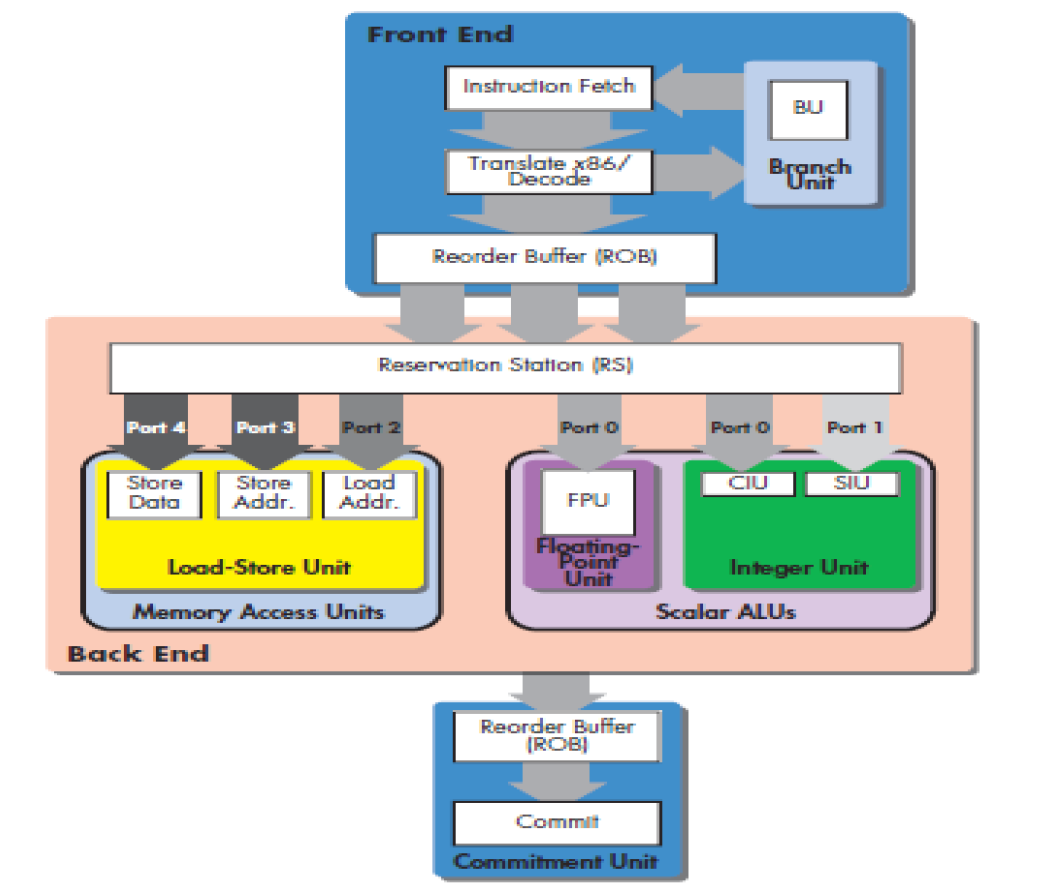
\includegraphics[width = 0.5 \textwidth]{images/11.PNG}
    \caption{Représentation Pentium Pro / Architecture P6}
  \end{figure}
\newpage
  Raison de l'abandon du Pentium original :
  \begin{itemize}
    \item S'adapte difficillement aux flux d'instructions dynamiques
    \item Exploite très faiblement l'hardware superscalaire "large"
    \item Ne pouvant dispatch que 2 instructions par cycle d’horloge, les règles de dispatch ont été conçues dans cette optique. Or, si plus d'unité, d'execution venaient à être disponnibles,
    les règles de dispatch devraient prendre en compte cet unité d'execution et donc de prendre en compte toutes les combinaisons possibles.
  \end{itemize}

  Solutions aux problèmes du Pentium Original :
  \begin{itemize}
    \item Dispatch des instructions décodées vers un buffer (un tampon) entre l'unité decode et les unités execute
    \item Quand le buffer possède un certain nombre d'instructions, la planification dynamique du processeur peut-être mis en place et évalué
    \item Il ne reste plus qu'a envoyer les instructions aux unités execute au moment le plus opportun et dans l'ordre optimal
    \item Comme avec ce système les instructions peuvent être dans le désordre par rapport au programme original, un tampon est placé a la sortie de son execution pour pouvoir
    permettre de les remettre dans l'ordre.
    \item L'opération qui consiste a placer les instruction dans le buffer \emph{issue} et de les envoyer dans les unitées d'execution une fois 
     que la planification dynamique aie été faite s'appelle le \emph{issuing}
  \end{itemize}

  \begin{figure}[H]
    \centering
    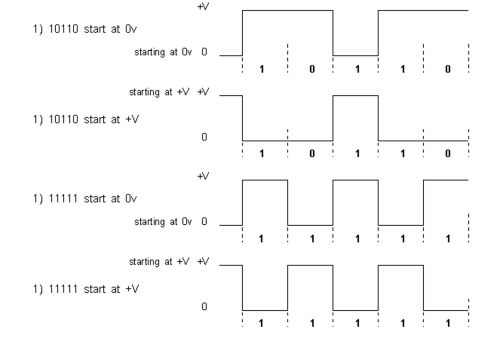
\includegraphics[width = 0.5 \textwidth]{images/12.PNG}
    \caption{Stratégie de planification dynamique}
  \end{figure}

  Pas toujours possible d'executer les instructions dans le désordre :
  \begin{itemize}
    \item Une instruction peut avoir comme entrée le résultat d'une instruction non execute
    \item Peut attendre des données venant de la mémoire
    \item Peut attendre que l'unité d'execution soit libre
  \end{itemize}

  Toute cette nouvelle stratégie s'appelle \emph{out-of-order execution} ou \emph{execution dynamique} :
  \begin{itemize}
    \item 2 nouvelles phases sont ajoutées
    \begin{itemize}
      \item Issue phase
      \item Completion phase
    \end{itemize}
  \end{itemize}

  \begin{figure}[H]
    \centering
    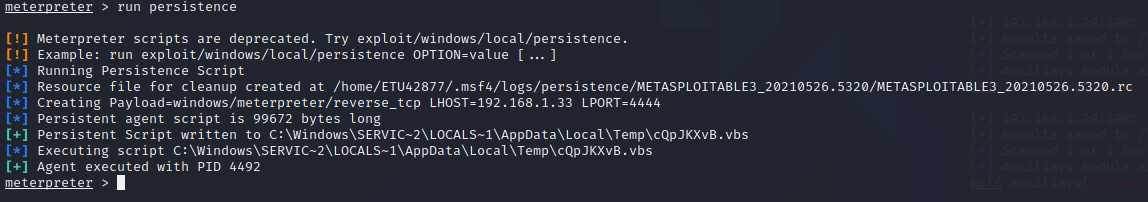
\includegraphics[width = 0.5 \textwidth]{images/13.PNG}
    \caption{Cycle de vie d'une instruction avec planification dynamique}
  \end{figure}

  \subsection{Issue Phase}
  \begin{itemize}
    \item Mise en tampon
    \item Réorganisation (on ne suit plus l'odre du programme)
    \item Peut comporter plusieurs étages de pipeline et/ou plusieurs tampons dépendant des processeurs
    \item Permet de réduire l'effet des bulles
  \end{itemize}

  \subsection{Completion Phase}
  \begin{itemize}
    \item Mise en tampon après l'execution
    \item Permet de remettre dans l'ordre prévu par le programme
    \item Permet l'illusion d'une exécution séquentielle
    \item Quand les résultats d'une instruction sont écrit dans le registre, on dit qu'elle est \emph{commit}
    \item Une instruction ne peut être commit tant que l'instruction la précédant n'est pas commit
  \end{itemize}

  \subsection{L'architcture P6}
  \subsubsection{Issue Phase}
  Le \emph{reservation station (RS)} est un buffer permettant d'acceuillir 3 instructions simultanément qui attendront que la condition de son execution soit validé, après quoi
  l'instruction est envoyée a l'unité d'execution (jusque 5 instructions pouvant être envoyé simultanément parce que 5 ports (voir \figurename{9})). 
  Comme dit plus haut, ici on ne suit plus l'odre du programme mais l'ordre 
  d'exécution optimal.
  \subsubsection{Completion phase}
  Pour pouvoir remettre les instructions dans l'odre, il est nécessaire de savoir dans quel ordre sont arrivées les instructions dans le \emph{reservation station}.
  C'est pour cela qu'on crée un \emph{recorder buffer (ROB)} juste avant d'entrer dans le \emph{RS} afin de pouvoir connaître le bon ordre de chaque instruction.
  \subsubsection{Pipeline}
  \begin{itemize}
    \item Branch Target Buffer (BTB) et Instruction Fetch : 3 niveau et $\frac{1}{2}$
    \item Decode : 2 niveau et $\frac{1}{2}$ (décoder les instructions x86 vers le format du processeur de type RISC)
    \item Register name : Registre renommés et instruction enregistrées dans le \emph{ROB} (1 cycle)
    \item Write to RS : Ecriture dans le reservation station (1 cycle)
    \item Read from RS : Issue phase en cours (peut rester dans le RS un nombre de cycle indéfini et la transition vers l'unité d'execution prends un cycle)
    \item Execute : Minimum 1 cycle
    \item Commit : 2 cycles (écrire dans le ROB puis remettre les résultats dans les registres)
  \end{itemize}
  
  Avantages de ce pipeline :
  \begin{itemize}
    \item $\uparrow$ fréquence d'horloge car étapes du pipeline plus courtes
    \item Pipeline avec un grand nombre d'instruction (problème si il faut vider le pipeline a cause d'une erreur de prédiction)
  \end{itemize}

  \subsubsection{Branch Prediction du P6}
  \begin{itemize}
    \item Précision des prédictions de 90\%
    \item 512 entrées du BHT + BTB et 4 bit pour les infos des prédictions passées
  \end{itemize}

  \subsubsection{RISC, CISC}
  \begin{itemize}
    \item La phase \emph{decode} est longue a cause de l'Instruction set Traduction
    \item Pour utiliser les techniques d'ordonnancement dynamique RISC, il fallai limiter la complexitée des instructions en traduisant les opérations x86 en opérations plus courtes 
    et plus à l'image du RISC.
    \item Mise en place d'une micro architecture de decodage qui utilise le microcode ROM pour les anciennes instructions CISC qui sont traduites en micro-opérations.
  \end{itemize}

  \begin{figure}[H]
    \centering
    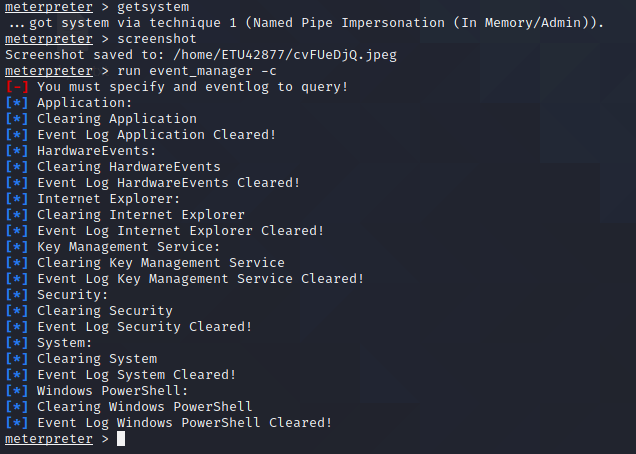
\includegraphics[width = 0.5\textwidth]{images/14.PNG}
    \caption{microarchitecture de decodage}
  \end{figure}

  Tout ce système d'heritage à un coût :\\
  \begin{itemize}
    \item 40\% de transistors pour ces opérations de decodage
  \end{itemize}























  \section{Processeurs 64 bits}
  
  Quand on parles d'un processeur étant de 16, 32, 64 bits; cela correspond au flux de données du processeur (nombre de bit que peut contenu chaque des registre du processeur).
  \begin{itemize}
    \item La largeur du flux de données a pu doubler
    \item La taille des bus et la taille des registres ont aussi doublé
  \end{itemize}

  Avantages :
  \begin{itemize}
    \item Dynamic Range (DR)
    \begin{itemize}
      \item On peut représenter beaucoup plus de nombre qu'en 32 bits
      \item Certaines applications nécessites des entiers à 64 bits
      \item Quand la valeur d'entier dépasse le nombre de bit max du processeur, on entre en situation d'overflow
      \begin{itemize}
        \item Quand ça arrive, le nombre donné est faux
      \end{itemize}
    \item Un bit permet de signaler si la DR a été dépassé pour prévenir les erreurs
    \end{itemize}
    
    \item Possibilitée d'utiliser dess adresses plus grandes
    \begin{itemize}
      \item La fourchette d'adresse s'appelle \emph{l'espace adressable}
      \item Tous les composants du PC avec lesquels on communique ont ainsi une adresse
    \end{itemize}

    \item En 32 bits, le proceseur et l'OS vont faire croire à un programme qu'il a un espace adressable de 4 Go ($2^{32}$). En 64 bits, 
    la théorie serait que cette espace soit de 18 millions de To ($2^{64}$) mais dans les faits c'est pas moins de 282To de mémoire virtuelle ($2^{48}$)
  \end{itemize}

  \tableofcontents































\end{document}